\setcounter{chapter}{0}
\chapter{Révisions}
\section{Quantité de matière: n}
	\subsection{Nombre d'Avogadro}
 		\blocrouge{Définitions}{La mole est une unité de quantité de matière. C'est un nombre de choses (par exemple: atomes, molécules ou ions).
Dans une mole, il y a $N_a$ (Nombre d'Avogadro) choses avec $N_a=\trou{\SI{6,02e23}{\per\mole}}$\\}


\subsection{Masse molaire}
	\blocrouge{Définition}{La masse molaire est la masse \trou{d'une mole}. \textit{c'est à dire la masse de $\SI{6,02e23}{}$ choses}.\\
Elle se note M et elle s'exprime en g/mol ou $\si{\gram \per  \mole}$.}

Pour une molécule, on la calcule à partir des masses molaires des atomes qui la compose.

\paragraph*{Remarque} Masse molaire atomique à connaître

\begin{tabular}{|l||c|c|c|c|}
	\hline
  Symbole de l'atome& C & H & O & N\\
  \hline
  M en g/mol& 12 & 1 & 16 & 14 \\
  \hline
\end{tabular}

Pour déterminer la quantité de matière d'un échantillon, on ne pourra évidemment pas compter les atomes ou les molécules. On pourra peser  l'échantillon et on calculera sa quantité de matière à l'aide de la relation:\\
\blocrouge{Formule}{$$\trou{\boxed{n=\frac{m}{M}}}$$ avec n en mol, m en g et M en $\si{\gram\per\mole}$}

\etiquette{Exercice }
On considère un échantillon de fer contenant $n=0,20$ mol.

\begin{enumerate}
    \item Calculer le nombre d'atomes de fer contenus dans cet échantillon.
    \item Calculer la masse de l'échantillon. On donne $M_{Fe}=56$ g/mol.
\end{enumerate}

\etiquette{Exercice} Quantité de matière d'une espèce moléculaire

Le glucose a pour formule brute: $C_6H_{12}O_6$.

\begin{enumerate}
    \item Exprimer puis calculer la masse molaire du glucose.
    \item Quelle est la quantité de matière contenue dans 20 g de glucose ?
\end{enumerate}

\subsection{Le volume molaire}
Le volume molaire est le volume d'une mole. Il se note $V_m$ et s'exprime en $\si{\liter\per\mole}$\\
Comme pour la masse, il existe une relation entre volume, volume molaire et quantité de matière.\\
\blocrouge{Formule}{$$\trou{\boxed{n=\frac{V}{V_m}}}$$   avec n en mol, V en L et $V_m$ en $\si{\liter\per\mole}$}

\blocrouge{Loi d'Avogadro-Ampère}{Pour les gaz, le volume molaire dépend de la pression, de la température, mais il est indépendant de la nature du gaz. C'est ce que l'on nomme la loi d'Avogadro-Ampère.\\
$V_m=\SI{24}{\liter\per\mole}$
}

\etiquette{Exercice} Quantité de matière d'un gaz

Il y a environ 4 L d'air dans nos poumons. Sachant que 20\% de cet air
est constitué de dioxygène, calculer la quantité de matière en dioxygène
présente dans nos poumons.
\subsection{Masse volumique et densité}

\blocrouge{Définitions}{
Un objet de masse $m$ qui occupe un volume $V$ a une masse volumique $\rho$ qui vaut$$\trou{\rho=\frac{m}{V}}$$
La densité d'un corps $d$ se calcule à l'aide de la masse volumique $\rho$ de ce corps et la masse volumique de l'eau $\rho_{eau}$ ainsi$$d=\frac{\rho}{\rho_{eau}}$$

}

\etiquette{Exemple}

La masse volumique du bois est 0,9 kg/L ce qui signifie qu'un objet en bois de 1 L pèse \trou{0,9 kg}.
Puisque 1L d'eau liquide pèse 1kg alors $\rho_{eau} = \trou{1}$ kg/L.
La densité du bois est \trou{$\frac{0,9\:kg/L}{1\:kg/L}=0,9$}. La densité est un nombre sans \trou{unité}.



\section{Solutions aqueuses}
\subsection{Vocabulaire}
Une solution est un soluté dissout dans \trou{un solvant} (ex : solution de café à partir de café soluble. La solution est obtenue par dissolution du café en poudre (le soluté) dans de l'eau (le solvant)).  \\
Le solvant est souvent de l'eau, on parle alors de solution aqueuse.\\
Une solution peut être plus ou moins concentrée. (un café fort et foncé sera plus concentré qu'un café doux et clair).\\

\subsection{Solutions ioniques}
Certains solides sont constitués d'un assemblage d'ions comme le chlorure de sodium (sel de cuisine) : $NaC\ell$ qui contient des ions $Na^+$ et $C\ell^-$. Dissoudre du sel dans l'eau revient à libérer et disperser les ions qu'il contient dans l'eau. Cette opération peut s'écrire à l'aide d'une équation de \trou{dissolution}:

$$NaC\ell(s) \longrightarrow Na^+(aq) + C\ell^-(aq)$$
Dans le cas du sulfate de sodium $Na_2SO_4$ on obtient:
$$Na_2SO_4(s) \longrightarrow 2 Na^+(aq) + SO_4^{2-}(aq)$$
Tous les solides ioniques comme toute la matière en général sont neutre \trou{électriquement}. 
Pour écrire une équation de dissolution, on doit connaître la formule des ions libérés. 

\etiquette{Ions à connaître}

\begin{tabular}{|l||c|c|c|c|c|l|}
	\hline
  Formule& $Na^+$ & $H^+$  & $C\ell^-$ & $SO_4^{2-}$ & $K^+$ &$MnO_4^{-}$\\
  \hline
  Nom& ion sodium & ion hydrogène & \trou{ion chlorure} & \trou{ion sulfate} & ion potassium&ion \trou{permanganate} \\
  \hline
\end{tabular}

\subsection{Concentration}
On définit la concentration massique et la concentration molaire : \\

\blocrouge{Définitions et Formules}{
\begin{itemize}\item
Concentration massique notée $c_m$: $$\trou{\boxed{c_m=\frac{m}{V}}}$$  \\
avec m la masse de soluté en g ; V le volume de la solution en L ; $c_m$ la concentration massique en $\si{\gram\per\liter}$\\
\item Concentration molaire notée $c$: $$\trou{\boxed{c=\frac{n}{V}}}$$   \\
avec n la quantité de matière de soluté en mol ; V le volume de solution en L ; $c$ la concentration molaire en $\si{\mole\per\liter}$\\
\\
\end{itemize}
}
\paragraph*{Remarques} Le volume de la solution n'est en général pas le même que le volume d'eau ajoutée au moment de la préparation de la solution. En général les exercices ne font pas cette distinction et on considère que le volume indiqué est celui de la solution. Si l'énoncé parle seulement de concentration sans préciser massique ou molaire alors on considère qu'il s'agit de concentration molaire.


\etiquette{Exercice} Concentration massique, molaire

On dissout 6,00 g de glucose dans 20 mL d'eau.

\begin{enumerate}
    \item Calculer la concentration massique puis molaire de la solution
    obtenue.
    \item On ajoute 20 mL d'eau à la solution, que vaut la nouvelle
    concentration molaire ?
\end{enumerate}

\etiquette{Exercice} Solide ionique et concentration en ions

On dissout une masse $m=3,0$ g de sulfate de sodium: $Na_2SO_4(s)$ dans de
l'eau. La solution obtenue a pour volume 100 mL et contient les ions
$Na^+$ et $SO_4^{2-}$. La masse molaire du sulfate de sodium est 142
g/mol.

\begin{enumerate}
    \item Écrire l'équation de dissolution du solide ionique $Na_2SO_4(s)$
    dans de l'eau.
    \item Calculer la concentration en soluté apporté notée C.
    \item Calculer la concentration en ions sodium $[Na^+]$ et la
    concentration en ions sulfate $[SO_4^{2-}]$. On donne $M_{Na}=23$
    g/mol et $M_{SO_4^{2-}}=96$ g/mol.
\end{enumerate}

\newpage
\etiquette{Exercice} Calcul de la concentration molaire d'une solution commerciale

Considérons une solution commerciale d'acide sulfurique ($H_2SO_4$) qui contient \SI{98}{\percent} en masse de $H_2SO_4$. La densité de cette solution est \SI{1.84}{g/mL}. La masse molaire de $H_2SO_4$ est \SI{98.1}{g/mol}.

\begin{enumerate}
    \item Calculer la masse totale de \SI{1.00}{L} de cette solution.
    \item Calculer la masse de $H_2SO_4$ dans \SI{1.00}{L} de cette solution.
    \item Déterminer la quantité de matière de $H_2SO_4$ dans \SI{1.00}{L} de cette solution.
    \item Calculer la concentration molaire de la solution d'acide sulfurique.
\end{enumerate}

\etiquette{Exercice } 
Considérons une solution commerciale d'acide nitrique $HNO_3$ qui contient \SI{68}{\percent} en masse de $HNO_3$. La densité de cette solution est \SI{1.42}{g/mL}. La masse molaire de $HNO_3$ est \SI{63.0}{g/mol}.

Prouver que la concentration molaire vaut \SI{15.3}{mol/L}

\section{Préparation de solution}
\subsection{Première technique: par dissolution}
\etiquette{Contexte et Matériel} 
\begin{itemize}
\item On dispose du soluté sous forme solide et de solvant.
\item On utilise une coupelle de pesée, une balance, une fiole jaugée et de l'eau distillée. 
\end{itemize}
\etiquette{Mise en Pratique}
\begin{figure*}[htp!]
	\begin{center}
		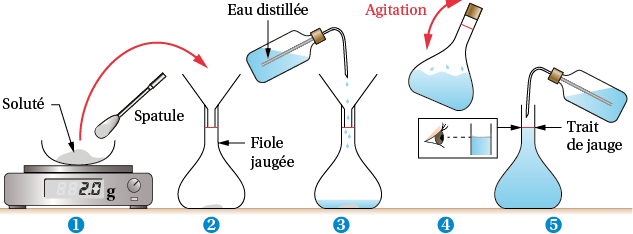
\includegraphics{figures/dissolution}
		\caption{Schéma de la dissolution}
	\end{center}	
\end{figure*}


\newpage
\subsection{Deuxième technique: par dilution}

\etiquette{Contexte et Matériel} 
\begin{itemize}
\item On dispose d'une solution concentrée: \trou{solution mère}. On veut préparer une solution de plus petite concentration: \trou{solution fille}. 
\item On prélève un volume de solution mère auquel on ajoute de l'eau de manière à abaisser la concentration. 
\item On utilise une\trou{ pipette jaugée}, une fiole jaugée et de l'eau distillée
\end{itemize}
\etiquette{Mise en Pratique}
\begin{figure*}[htp!]
	\begin{center}
		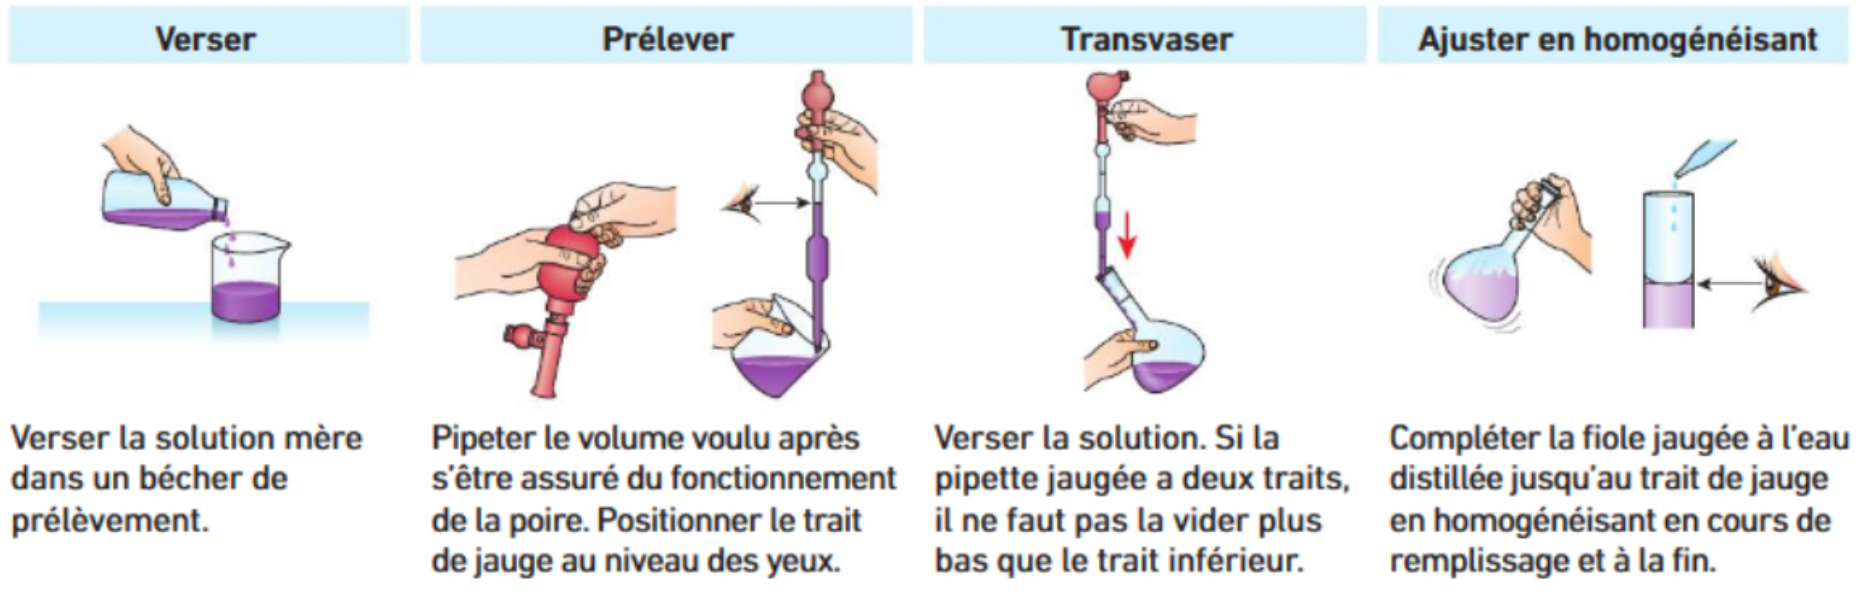
\includegraphics[width=1\textwidth]{figures/dilution}
		\caption{Schéma de la dilution}
	\end{center}	
\end{figure*}

\subsection{Calculs de dilution}

Pour effectuer une dilution, on doit calculer le volume de solution mère à prélever. Cela nous donne aussi le volume de la pipette jaugée à utiliser. Pour faire ce calcul, on utilise le\trou{ facteur de dilution}.
%\paragraph*{Conservation de la matière}
%
%On dispose d'une solution d'eau salée à $C_1= 10$ g/L. On veut préparer $V_2=50$ mL de solution d'eau salée à $C_2= 4,0$ g/L. 
%
%\etiquetterouge{Idée} La quantité de solution présente dans la solution fille de  volume $V_2$ est exactement contenue dans le petit volume \trou{$V_1$ } de solution mère prélevée.
%
%Il y a la même quantité de soluté dans la solution fille de concentration $C_2$ et de volume $V_2$ que dans le prélèvement de solution mère de volume $V_1$ et de concentration $C_1$. Faire un schéma de cette phrase.
%
%On a donc:$$\trou{C_1\times V_1 = C_2\times V_2}$$ Le volume à prélever cherché est $$V_1=\frac{C_2.V_2}{C_1}$$

\blocrouge{Définition}{Le facteur $F$ de dilution est le rapport entre la concentration de la solution mère $C_1$ et la concentration de la solution fille $C_2 < C_1$. C'est aussi le rapport entre le volume de la solution fille et le volume de solution mère à prélever (volume de la pipette)$$\trou{F=\frac{C_1}{C_2}=\frac{V_2}{V_{pipette}}}$$
}

\blocgris{Exemple important}{
On dispose d'une solution d'eau salée à $C_1= 10$ g/L. On veut préparer $V_2=50$ mL de solution d'eau salée à $C_2= 4,0$ g/L. Calculer $V_1$ en utilisant la méthode du facteur de dilution.
\vspace{8cm}}
 
 \etiquette{Exercice} Dissolution et Dilution

On dispose de chlorure de sodium solide ($NaC\ell$). On souhaite
réaliser une solution $S_1$ de volume $V_1=50$ mL et de concentration
$C_1=\SI{1.50e-2}{\mol\per\liter}$. La masse molaire du chlorure de
sodium est 58,5 g/mol.

\begin{enumerate}
    \item Indiquez le protocole expérimental permettant de réaliser la solution $S_1$. On fera un schéma, un calcul et des phrases.
    \item A partir de $S_1$, on prépare une solution $S_2$ de volume $V_2=75,0$ mL et de concentration de $C_2=\SI{5.00e-3}{\mol\per\liter}$. Détailler le protocole expérimantal qui conduit à l'élaboration de $S_2$. On fera la liste du matériel et des schémas clés.
\end{enumerate}

 \section{Transformations chimiques}
 \subsection{C'est quoi une transformation chimique ?}
 Parfois lorsque l'on met en contact deux substances chimiques, elles se transforment en de nouvelles substances.  On parle de transformation chimique. Les substances présentes au début, s'appellent les\trou{ \textbf{réactifs}}. Ils sont consommés au cours de la réaction. Les nouvelles substances qui apparaissent sont appelées \trou{\textbf{produits}}. 

 \subsection{Comment ça s'écrit ?}
 On modélise la transformation par une équation de réaction. \\

\blocgris{Exemple pas à pas}{ 
Le propane ($\mathrm{C_3H_8}$) réagit avec le dioxygène pour donner du dioxyde de carbone et de l'eau. Comment écrire l'équation chimique de cette transformation ?\\
\begin{enumerate}
	\item Faisons la liste des réactifs et des produits.
\\
Initialement les espèces présentes sont les réactifs: $C_3H_8$ et $O_2$. Celles qui aparaissent sont $CO_2$ et $H_2O$	
	
	\item Proposer une écriture de l'équation de le réaction.\\
On commence par écrire:$$C_3H_8 + O_2 \longrightarrow CO_2 + H_2O$$
\item On ajoute des \textbf{coefficients stoechiométriques} pour valider les 2 principes importants (ci-dessous)
 $$\trou{3}\times\boxed{C_3H_8} + \trou{5}\times\boxed{O_2} \longrightarrow \trou{3}\times\boxed{CO_2} + \trou{4}\times\boxed{H_2O}$$\\
 Ce qu'on écrit simplement:
 $$C_3H_8 + ...O_2 \longrightarrow 3CO_2 + ...H_2O$$
\end{enumerate}
}
\paragraph*{Lecture d'une équation chimique} Lorsque 3 moles de propane sont consommées cela consomme aussi 5 moles de $O_2$. La réaction produit alors 3 moles de $CO_2$ et 4 moles d'eau.

\blocrouge{2 Principes importants}{
Une équation chimique est équilibrée si elle vérifie:
\begin{enumerate}
\item La conservation de chaque élément chimique.
\item La conservation de \trou{la charge} (charge de l'ensemble des réactifs = charge de l'ensemble des produits). 
\end{enumerate}
}

 \subsection{Méthode du tableau d'avancement}
Pour décrire quantitativement la transformation chimique, on considère 3 états particuliers:
\begin{enumerate}
	\item L'état initial: les réactifs n'ont pas encore réagi. L'avancement x vaut 0 mol.
	\item L'état intermédaire: la réaction a commencé à se faire mais n'est pas terminée.  $0<x<x_f$
	\item L'état final: Les quantités de matière n'évoluent plus. L'avancement a atteint sa dernière valeur: $x_f$
\end{enumerate}

\blocgris{Exemple pas à pas}{
On fait réagir 1 mol de $H_2$ avec 2 mol d'$O_2$. Le produit obtenu est de l'eau. Cette réaction est \textbf{totale}. On cherche la quantité de matière d'eau que va produire cette réaction.\\
Nou construisons un tableau d'avancement :\\
		\begin{center}
		\begin{tabular}{|l|c|c|c|c|}
\hline 
  \multicolumn{2}{|c!{\protect\makebox[0cm]{:}}}{\textbf{Equation chimique}} &
 \multicolumn{1}{c!{\makebox[0cm]{+}}}{%
      $\mathrm{2H_2(g)}$} &
       \multicolumn{1}{c!{\protect\makebox[0cm]{$\rightarrow$}}}{%
      $\mathrm{O_2(g)}$} &
       \multicolumn{1}{c|}{%
      $\mathrm{2H_2O(g)}$} 
	 
%\tabularnewline
\\
\hline 
Etat du système&
avancement& $\mathrm{n_{H_2}}$ 
&$\mathrm{n_{O_2}}$  
&$\mathrm{n_{H_2O}}$ 

\tabularnewline
\hline 
Etat initial&
$x=0$&.....
&.....
&.....

\tabularnewline
\hline 
Etat intermédiaire&
$x$&$....$
&$....$
&$....$

\tabularnewline
\hline 
Etat final&
$x=x_{f}$&$....$
&$.....$
&$.....$
\tabularnewline
\hline
\end{tabular}
\end{center}
\begin{enumerate}
	\item On relève les quantités matière initiales et on les place à la première ligne du tableau.
	\item A l'état intermédiaire, le contenu des cases est de la forme $n_{initial}-CoeffStoechio\times x$ pour les réactifs et $CoeffStoechio\times x$ pour les produits.
	\item Idem état intermédiaire en remplaçant $x$ par sa valeur particulière $x_f$.
\end{enumerate}

Cela donne 
		\begin{center}
		\begin{tabular}{|l|c|c|c|c|}
\hline 
  \multicolumn{2}{|c!{\protect\makebox[0cm]{:}}}{\textbf{Equation chimique}} &
 \multicolumn{1}{c!{\makebox[0cm]{+}}}{%
      $\mathrm{2H_2(g)}$} &
       \multicolumn{1}{c!{\protect\makebox[0cm]{$\rightarrow$}}}{%
      $\mathrm{O_2(g)}$} &
       \multicolumn{1}{c|}{%
      $\mathrm{2H_2O(g)}$} 
	 
%\tabularnewline
\\
\hline 
Etat du système&
avancement& $\mathrm{n_{H_2}}$ 
&$\mathrm{n_{O_2}}$  
&$\mathrm{n_{H_2O}}$ 

\tabularnewline
\hline 
Etat initial&
$x=0$&1&2&0

\tabularnewline
\hline 
Etat intermédiaire&
$x$&1-2x&2-x&2x
\tabularnewline
\hline 
Etat final&
$x=x_{f}$&$1-2x_f$
&$2-x_f$
&$2x_f$
\tabularnewline
\hline
\end{tabular}
\end{center}
}


Lorsque la réaction est totale, elle continue à se faire jusqu'à ce qu'un des réactifs soit entièrement consommé. 

\blocrouge{A retenir}{

\begin{itemize}
	\item Par définition, le réactif est entièrement consommé à l'état final et s'appelle \textbf{réactif limitant}.
	\item Si la réaction est \textbf{totale} et on a: \\ \boxed{ $$\trou{x_f = x_{max}}$$}.
\end{itemize}
}

Voyons la méthode pour calculer $x_{max}$:

\blocgris{Exemple pas à pas}{
\paragraph*{Hypothèse 1:} le $H_2$ est le réactif limitant 
Alors $1-2x_{max}=0$ et $x_{max}= ... \si{\mole}$\\
\paragraph*{Hypothèse 2:}  $O_2$ est le réactif limitant 
Alors $2-x_{max}=0$ et $x_{max}=$\\
Nous garderons \textbf{toujours la plus petite valeur} de $x_{max}$. \\
Dans notre exemple, on aura donc $x_{max}=.....$ et $H_2$ est le réactif limitant.\\
\paragraph*{Bilan de matière à l'état final}
On remplace $x_f$ par la valeur de $x_{max}$ que l'on vient de calculer dans toutes les cases de l'état final.
On trouve: 

		\begin{center}
		\begin{tabular}{|l|c|c|c|c|}
\hline 
  \multicolumn{2}{|c!{\protect\makebox[0cm]{:}}}{\textbf{Equation chimique}} &
 \multicolumn{1}{c!{\makebox[0cm]{+}}}{%
      $\mathrm{2H_2(g)}$} &
       \multicolumn{1}{c!{\protect\makebox[0cm]{$\rightarrow$}}}{%
      $\mathrm{O_2(g)}$} &
       \multicolumn{1}{c|}{%
      $\mathrm{2H_2O(g)}$} 
	 
%\tabularnewline
\\
\hline 
Etat du système&
avancement& $\mathrm{n_{H_2}}$ 
&$\mathrm{n_{O_2}}$  
&$\mathrm{n_{H_2O}}$ 

\tabularnewline
\hline 
Etat initial&
$x=0$&1&2&0

\tabularnewline
\hline 
Etat intermédiaire&
$x$&1-2x&2-x&2x
\tabularnewline
\hline 
Etat final&
$x=x_{f}=x_{max}= 0,5$&$1-2\times 0,5 = 0$
&$2-0,5=1,5$
&$2\times 0,5=1 $
\tabularnewline
\hline
\end{tabular}
\end{center}
}

A l'aide de la méthode du tableau d'avancement, on prédit qu'à l'état final le système chimique aura la composition suivante:
\begin{itemize}
	\item $\mathrm{n_f(H_2)}=1-2\times0,5=\SI{0}{\mole}$
	\item $\mathrm{n_f(O_2)}=2-0,5=\SI{1.5}{\mole}$
	\item $\mathrm{n_f(H_2O)}=2\times0.5=\SI{1}{\mole}$
\end{itemize}

\paragraph*{Remarques}
\begin{itemize}
	\item Lorsque la réaction n'est pas totale, à l'état final \trou{$x_f < x_{max}$} et au lycée il n'y a pas de méthode générale pour prédire sa valeur. Une réaction non totale est aussi appelée: équilibre chimique et l'état final est l'état d'équilibre (nous étudierons cela dans le prochain chapitre).
	\item En faisant réagir 2 mol de $H_2$ avec 1 mol de $O_2$ on produit 2 mol de $H_2O$ et il ne reste ni $H_2$ ni $O_2$. Cet état initial particulier s'appelle \trou{mélange stoechiométrique}. Il permet de consommer la totalité de tous les réactifs. Il intervient aussi à l'équivalence des titrages.
\end{itemize}

\blocrouge{Mélange Stoechiométrique}{Soit une équation chimique : $$ aA+bB\longrightarrow cC $$ a,b et c sont les coefficients stoechiométriques des espèces chimiques A, B et C. On note $n_A$ la quantité de matière initiale de A et $n_B$ la quantité de matière de B. Le mélange est stoechiométrique si l'égalité suivante est vérifiée:
  $$\frac{n_A}{a}=\frac{n_B}{b}$$ }


\etiquette{Exercice }

Considérons la réaction chimique suivante :
 $$2 A\ell_{(s)} + 3 C\ell_{2(g)} \longrightarrow 2 A\ell C\ell_{3(s)}$$

On mélange \SI{3.0}{mol} d'aluminium avec \SI{4.0}{mol} de dichlore à l'état gazeux .

\begin{enumerate}
    \item Écrire le tableau d'avancement de cette réaction.
    \item Déterminer l'avancement maximal de la réaction.
    \item Calculer les quantités de matière des réactifs et des produits à l'état final.
    \item Identifier le réactif limitant et le réactif en excès.
    \item Calculer la masse de produit.
\end{enumerate}
 \newpage
 
 \etiquetterouge{Important}
 QR Code des documents partagés sur Google Drive
 \begin{center}
	 
\includegraphics[scale=.4]{figures/qrcode_video_1} 	
 \end{center}

 
 \vspace{2cm}
 
 \blocoval{Essentiels}
 {
 \begin{tabular}{l|l}
 A connaître & Techniques  \\
  \hline
Définitions  & Calculer la quantité de matière à partir de la masse \\
        & Calculer la quantité de matière d'un gaz\\
 Masse volumique&Savoir utiliser la formule\\
 &Distinguer $d$ et $\rho$\\       
Concentration massique et molaire& Equation de dilution\\
& Calculs de concentration\\
Dissolution& Protocole \\
& Calcul de la masse de soluté à peser\\
Dilution& Protocole\\
& Calcul du volume de solution mère à prélever\\
Equation chimique& Savoir équilibrer\\
 & Lecture en terme de consommation et production\\
 Tableau d'avancement & Savoir appliquer la méthode\\ 
 &Déterminer $x_{max}$  et l'état final\\
 Mélange stoechiométrique&Justifier qu'un mélange intial est stoechiométrique

\end{tabular}
 }
 